\documentclass[10pt,conference,letterpaper]{IEEEtran}
\usepackage{verbatim}
\usepackage{moreverb}
\usepackage{url}
\usepackage{amsmath}
\usepackage{color}

\title{HAMAKE: A Dataflow Approach to Data Processing in Hadoop}

\author{\IEEEauthorblockN{Vadim Zaliva}
\IEEEauthorblockA{Codeminders\\
Email: lord@crocodile.org} \and \IEEEauthorblockN{Vladimir Orlov}
\IEEEauthorblockA{Codeminders\\
Email: vorl@codeminders.com}}

\date{\today}
\usepackage{graphicx}
\usepackage{listings}
\usepackage{rotating}
\usepackage[colorlinks=false,bookmarks=true,pdfauthor={Vadim Zaliva lord@crocodile.org, Vladimir Orlov vorl@codeminders.com},
            pdftitle={HAMAKE: A Dataflow Approach to Data Processing in Hadoop},
            pdftex]{hyperref}

% graphviz.tex
% originally written by Derek Rayside, November 2003
% following an idea that Daniel Jackson implemented in his Tagger program
%
% parameters to \digraph:
% 1 - parameters for \includegraphics (optional; default value is "scale=1")
% 2 - name of the digraph
% 3 - body of the digraph

\newcommand{\digraph}[3][scale=1]{
    \newwrite\dotfile
    \immediate\openout\dotfile=#2.dot
    \immediate\write\dotfile{digraph #2 {\string#3}}
    \immediate\closeout\dotfile
    \IfFileExists{#2.ps}
        % the postscript exists: include it
        { \includegraphics[#1]{#2} }
        % the postscript doesn't exist: tell the user how to create it
        { \fbox{ \begin{tabular}{l}
            The file \texttt{#2.ps} hasn't been created from
            \texttt{#2.dot} yet. \\
            Run `\texttt{dot -Tps -o #2.ps #2.dot}' to create it. \\
            Here is a \textsf{bash} loop to process all \textsf{dot} files
            in the current directory: \\
            \texttt{
            for f in *.dot do ; 
            dot -Tps -o \$\{f\%dot\}ps \$f ; 
            done
            }
            \end{tabular}}
        }
}


\begin{document}
\lstset{language=XML,basicstyle=\tiny,markfirstintag=true,numbers=left,numbersep=1pt}

\maketitle

\begin{abstract}
  Most non-trivial data processing scenarios using Hadoop typically
  involve launching more than one MapReduce job. Usually, such
  processing is data-driven, with the data funneled through a sequence
  of jobs.  The processing model could be expressed in terms of
  dataflow programming, represented as a directed graph with datasets
  as vertices. Using \textit{fuzzy timestamps} as a way to detect
  which dataset needs to be updated, we can calculate a sequence in
  which Hadoop jobs need to be launched to bring all datasets up to
  date. Incremental data processing and parallel job execution fit
  well into this approach.

  These ideas inspired the creation of the \textbf{hamake} utility. We
  attempted to emphasize data and allowing the developer to formulate
  his or her problem as a data flow (as opposed to the workflow
  approach commonly used). \textbf{Hamake} language uses just two data
  flow operators: \emph{fold} and \emph{foreach}, providing a clear
  processing model similar to MapReduce, but on a dataset level.
\end{abstract}

\section{Motivation and History}

MapReduce data processing model have been introduced by
Google\cite{dean2008map}. Hadoop\cite{bialecki2005hadoop} is a popular
open-source implementation of MapReduce.

Hadoop is typically used to process big amounts of data via series of
relatively simple operations. Usually Hadoop jobs are I/O-bound
\cite{hadoopattwitter},\cite{hs2010hadoopbench}, and execution of even
trivial operations on a large dataset could take significant system
resources. This makes incremental processing important. Our initial
inspiration was the Unix \emph{make} utility. While applying some of the same ideas implemented by \emph{make}
to Hadoop, we took an opportunity to generalize the
processing model in terms of dataflow programming.

\textbf{Hamake} was developed in late 2008 to address the problem of
incremental processing of big data sets in a collaborative filtering
project.

We've striven to create a simple-to-use utility that developers can
start using right away without complex installation or an extensive
learning curve. 

\textbf{Hamake} is open source, distributed under Apache
License v2.0. The project is hosted at Google Code at the following
URL: \url{http://code.google.com/p/hamake/}.

\section{Processing Model}

\textbf{Hamake} operates on \textit{files}, residing on a local or
distributed file system accessible from the Hadoop job (usually it is
HDFS). Each file has a timestamp, reflecting the date and time of its
last modification. A file system directory or folder is also a file,
and has its own timestamp. A \textit{Data Transformation Rule (DTR)}
defines an operation which takes files as input and produces other
files as output.

If file \textit{A} is listed as input of a DTR, and file \textit{B}
listed as output of the same DTR, it is said that \textit{``B depends
  on A''}. \textbf{Hamake} uses file time stamps for dependency
up-to-date checks. DTR output is said to be \textit{up to date} if the
minimum time stamp on all output is greater or equal to the maximum
timestamp on all input. For the sake of convenience, a user could
arrange groups of files and folders into a \emph{fileset} which later
could be referenced as the DTR's input or output.

\textbf{Hamake} uses \textit{fuzzy timestamps}\footnote{Current stable
  version of \textbf{hamake} uses exact (non-fuzzy) timestamps.}
which could be compared, allowing for a certain margin or error. The
``fuzziness'' is controlled by tolerance $\sigma$. Timestamp $a$ is
considered to be older than timestamp $b$ if $(b-a)>\sigma$. Setting
$\sigma=0$ gives us non-fuzzy, strict timestamp comparison.

\textbf{Hamake} attempts to ensure that all output from a DTR are up to
date\footnote{\textbf{hamake} does not try to ensure that files which
  are not listed as one of a DTR's output are up to date, because it has
  no way to update them.}.  To do so, it builds a \textit{dependency
  graph}. This graph has individual files or filesets as vertices and
DTRs as edges. Below, we will show that this graph is guaranteed to be
a \textit{Directed Acyclic Graph} (DAG).

After building a \textit{dependency graph}, a graph reduction algorithm (shown in Figure~\ref{fig:grred}) is
executed. Step 1 makes use of Kahn's algorithm\cite{kahn1962topological} of
topological ordering. In step 6, when the completed DTR is
removed from the dependency graph, all edges pointing to it from other
DTRs are also removed.

\begin{figure}[htp]
\centering
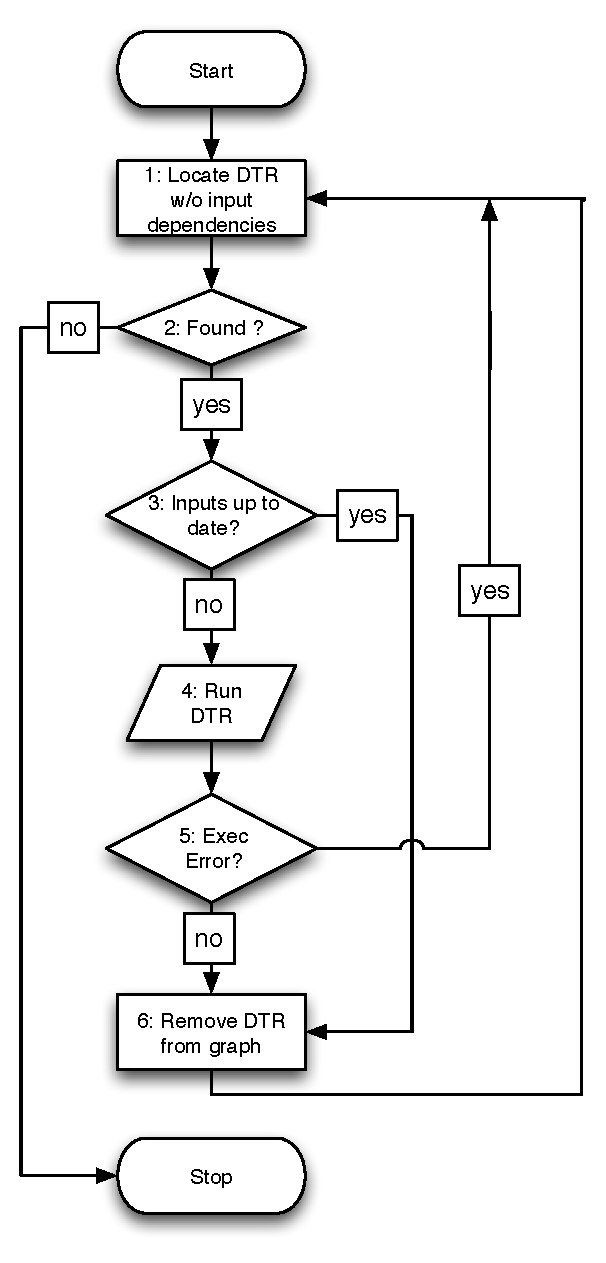
\includegraphics[width=4cm]{GraphReduction.eps}
\caption{\textbf{hamake} dependency graph reduction algorithm}
\label{fig:grred}
\end{figure}

The algorithm allows for parallelism. If more than one DTR without
input dependencies is found during step 1, subsequent steps 2-6 could
be executed in parallel for each discovered DTR.

It should be noted that if DTR exectuion has failed, \textbf{hamake} can
and will continue to process other DTRs which do not depend directly or indirectly
on the results of this DTR. This permits the user to fix problems later and
re-run \textbf{hamake}, without the need to re-process all data, saving valuable time.

Cyclic dependencies must be avoided, because a dataflow containing
such dependencies is not guaranteed to terminate. Implicit checks are
performed during reading DAG definitions and building the dependency
graph. If a cycle is detected, it is reported as an error. Thus the
dependency graph used by \textbf{hamake} is ensured to be a
\textit{directed acyclic graph}.

However \textbf{hamake} supports a limited scenario of iterative
processing via a feature called \textit{generations}. Each input or
output file has the option to be marked with a \emph{generation}
attribute. Two files with different generation numbers while
referencing the same path in the file system are treated as different
vertices in the dependency graph. This allows for the resolution of cyclic dependencies
in the context of a single \textbf{hamake} execution.

One useful consequence of \textbf{hamake} dataflow being a DAG is
that for each vertex we can calculate list of vertices it depends on,
directly and indirectly using simple \textit{transitive closure}. On
datasets, where the cost of re-calculation could be potentially high
(due to data size or computational complexity) this allows us to estimate
the scope of a dataflow graph affected by updating one or more files.

\textbf{Hamake} is driven by dataflow description, expressed in simple
XML-based language. The full syntax is described in
\cite{hamakesyntax}. The two main elements, \emph{fold} and \emph{foreach},
 correspond to two types of DTRs. Each have input,
output and processing instruction. Executing processing instruction
should bring DTR output up to date, compared to its
input. \emph{Fold} implies a many-to-one dependency between input and
 output. In other words, output depends on the entirety of the input, and if
any input has been changed, the output needs to be
updated. \emph{Foreach} implies one-to-one dependency: where for each
file in an input set there is a corresponding file in an output set, each updated independently.

\textbf{Hamake} dataflow language has a declarative semantics. Keeping it
purely declarative makes it easy to implement various
dataflow analysis and optimization algorithms on top of it in the future. Some
examples of such algorithms could be: merging dataflows, further
execution parallelization, dataflow complexity analysis and
estimation.

\section{Parallel Execution}

While determining the sequence and launching Hadoop jobs required to
bring all datasets up-to-date, \textbf{hamake} attempts to perform all
required computations in the shortest possible time. To achieve this, it
aims for maximal cluster utilization, running as many Hadoop jobs in
parallel as cluster capacity permits.

There are three main factors driving job scheduling logic: file
timestamps, dependencies, and cluster computational capacity. On the
highest level DTR dependencies determine the sequence of DTR jobs being
launched.

In the case of \emph{fold} DTR, a single Hadoop job, PIG script or shell
could be launched and hence there are not many opportunities for
parallel execution. In the example shown in Figure~\ref{fig:fold2}, since
fileset \textit{B} depends on all files in fileset \textit{A}, a
single job associated with \emph{fold} DTR will be executed.

\begin{figure}[htp]
\centering
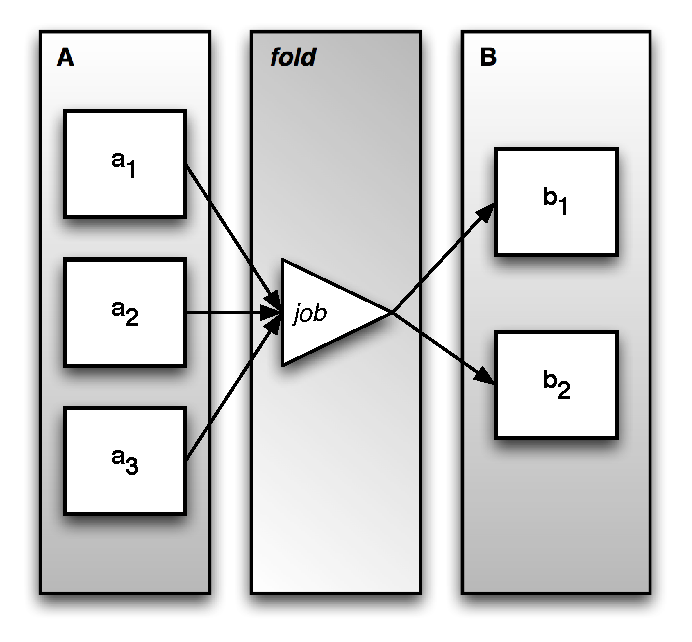
\includegraphics[width=0.3\textwidth]{twofoldp.eps}
\caption{Simple \emph{fold} DTR}
\label{fig:fold2}
\end{figure}

A \emph{foreach} DTR works by mapping individual files in fileset
\textit{A} to files in fileset \textit{B}. Assuming that fileset
\textit{A} consists of 3 files: \textit{$a_1$}, \textit{$a_2$},
\textit{$a_3$} the the dependency graph could be represented as shown
in Figure~\ref{fig:foreach2}. In this case we have an opportunity to
execute three jobs in parallel.

\begin{figure}[htp]
\centering
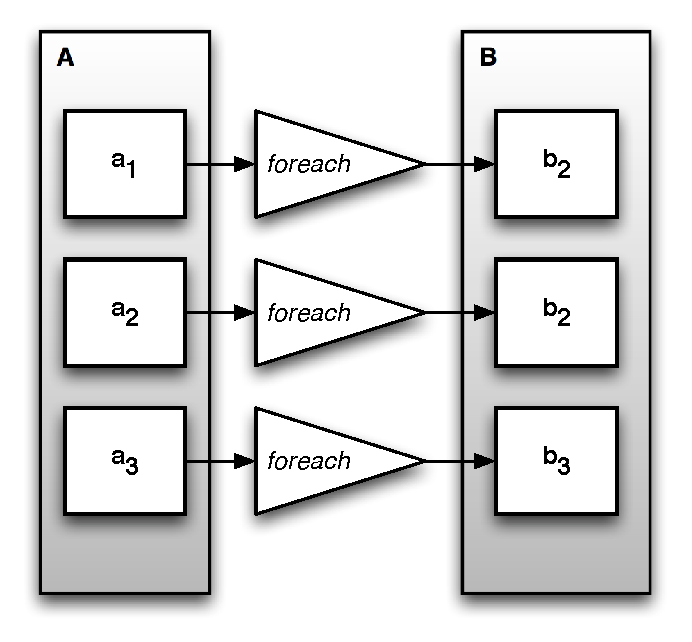
\includegraphics[width=0.3\textwidth]{twoforeachp.eps}
\caption{Decomposition of \emph{foreach} DTR}
\label{fig:foreach2}
\end{figure}

The Hadoop cluster capacity is defined in terms of the number of
\textit{map slots} and \textit{reduce slots}. When a DTR launches a Hadoop job
(either directly as defined by \emph{mapreduce} processing instruction
or via PIG script), a single job will spawn one or more \emph{mapper}
and \emph{reducer} tasks, each taking one respective slot. The number of
mappers and reducers launched depends on many factors, such as size of the
HDFS block, Hadoop cluster settings, and individual job settings. In
general, \textbf{hamake} has neither visibility of nor
control over most of these factors, so the \textbf{hamake} scheduler
currently does not deal with individual tasks. Thus \textbf{hamake}
parallel execution logic is controlled by a command line option
specifying how many jobs it is allowed run in parallel.

\section{Example}

Let us consider a hypothetical example demonstrating \textbf{hamake}
use. Imagine an online library containing digital copies of millions of
books. Considering the size of such a library, it's hardly surprising that
there are duplicated titles in it. Such duplicates may be caused by
OCR errors, typos, differences in formatting, or added material such
as a foreword or publisher information.

For the purpose of illustrating \textbf{hamake} usage, we will
consider the simple approach of using a \textit{vector space
  model}\cite{manning2008introduction} based on word frequencies and
\textit{Canopy clustering algorithm}\cite{efficientClustering}. The
implementation could be split into a series of steps, each of them
represented by a \textit{MapReduce job}:

\begin{description}[\IEEEsetlabelwidth{\emph{FilterStopwords}}]
\item[\emph{ExtractText}] Extract a plain text from native document format
  (e.g. PDF).
\item[\emph{Tokenize}] Split plain text into a tokens, roughly
  corresponding to words. Dealing with hyphens, compound words,
  accents and diacritics, case-folding, stemming or lemmatization of
  tokens, resulting in a list of normalized \text{tokens}.
\item[\emph{FilterStopwords}] Filtering out \textit{stopwords} (e.g. words
  like \textit{a}, \textit{the}, \textit{are}) from the list of
  terms.
\item[\emph{CalculateTF}] For each document calculate a feature
  vector: a vector of term frequencies.
\item[\emph{FindSimilar}] Run \textit{Canopy clustering algorithm}
  for grouping similar books in clusters. Use
  \textit{cosine distance} as a fast approximate distance metric. 
\item[\emph{OutputResult}] Output book names, which are found in
  clusters with more than one elements
\end{description}

Each of the resulting six MapReduce jobs produces an output file which
depends on its input. For each book, these jobs must be invoked
sequentially, as the output of one task is used as input of the next. Additionally, there is a configuration file containing a list of
stop words, and some tasks' output depend on this file content. These
dependencies could be represented by a directed acyclic graph, shown in
Figure~\ref{fig:SimilarityAlgDAG}, with vertices representing data
files, and jobs assigned to edges. The XML file describing the
dataflow in \textbf{hamake} language is show as
Listing~\ref{hamakeFile}.

\lstinputlisting[caption={\textit{hamakefile}, that describes process for
  detecting similar books}, label=hamakeFile]{sample.xml}

The first DTR (lines 10-25) converts a book from a native format such
as PDF to plain text. The input of the DTR is a reference to the
\emph{/doc} folder, and the output is the \emph{/txt} folder. The
\emph{foreach} DTR establishes one-to-one dependency between files
with the same names in these two folders. The Hadoop job which
performs the actual text extraction is defined using the \emph{mapreduce}
element. It will be invoked by \textbf{hamake} for each unsatisfied
file dependency. The job takes two parameters, defined with
\emph{parameter} elements - a path to a book as the input, and a path to a
file, where the plain text version should be written. The remaining five
DTRs are defined in a similar manner.

\textbf{Hamake}, when launched with this XML dataflow definition, will
first search for DTRs that have no input or for which the input is not also the
output of other tasks. In our particular example, this is
\emph{ExtractPlainText}. \textbf{Hamake} will launch corresponding
Hadoop jobs first, and as soon as they are finished, it will
execute DTRs which depend on the output of this DTR, and so on until all
output files are up to date. As a result of this data flow, a file
\emph{results.txt} with list of similar books will be generated.

This data flow could be used for incremental processing. When new
books are added, \textbf{hamake} will not re-run the following DTRs:
\emph{ExtractText}, \emph{Tokenize}, \emph{FilterStopWords}, and
\emph{CalculateTF} for previously processed books. However it will run
these DTRs for newly added books, and then, will re-run
\emph{FindSimilar} and \emph{OutputResults}.  If the list of stop
words has been changed, \textbf{hamake} will re-run only
\emph{FilterStopWords} \emph{CalculateTF}, \emph{FindSimilar}, and
\emph{OutputResults} DTRs.

\begin{figure}[htp]
\centering
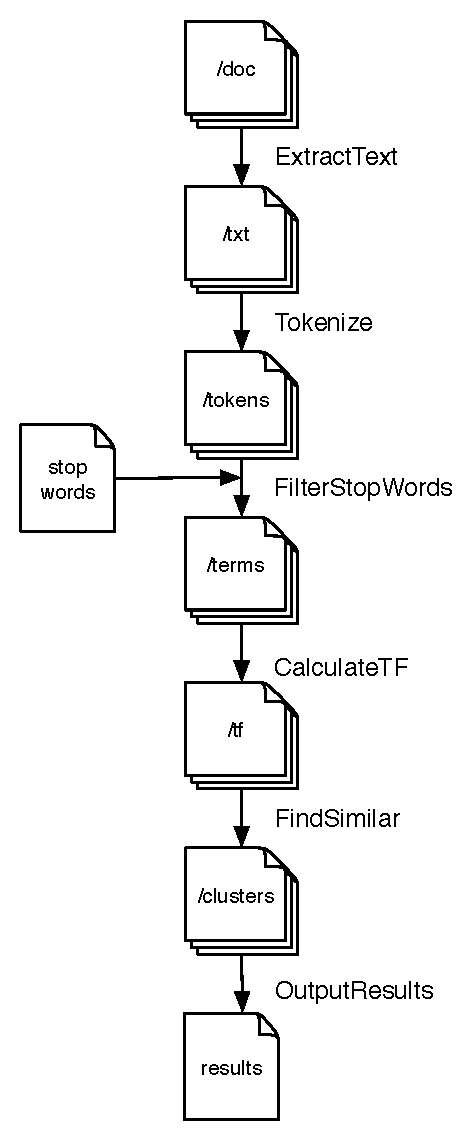
\includegraphics[width=0.25\textwidth]{SimilarityAlgDAG.eps}
\caption{Directed Acyclic Graph of a similar books detection data flow}
\label{fig:SimilarityAlgDAG}
\end{figure}

\section{Related Work}

Several workflow engines exist for Hadoop, such as
\href{http://github.com/tucu00/oozie1}{Oozie},
\href{http://sna-projects.com/azkaban/}{Azkaban}, and
\href{http://www.cascading.org/}{Cascading}.  Although all of these
products could be used to solve similar problems, they differ
significantly in design, philosophy, target user profile, usage
scenarios, etc., limiting the usefulness of simple feature-wise
comparison.

The most significant difference between these engines and \textbf{hamake}
lies in the \textit{workflow} vs. \textit{dataflow} approach. All of them
use the former, explicitly specifying dependencies between
jobs. \textbf{Hamake}, on the other hand, uses dependencies between datasets
to derive workflow. Both approaches have their advantages. One
could argue that for some problems, the dataflow representation as used by
\textbf{hamake} is more natural.

\section{Future Directions}

One possible \textbf{hamake} improvement may be developing better integration with
Hadoop schedulers. For example, if \textit{Capacity Scheduler} or
\textit{Fair Scheduler} is used, it would be useful for \textbf{hamake} to take into account
information about its \textit{pools} or \textit{queues} capacities in a
job scheduling algorithm.

More granular control over parallelism could be achieved if the
\textbf{hamake} internal dependency graph contained individual
files, not just DTRs. For example, consider a dataflow consisting of
three datasets \textit{A}, \textit{B}, \textit{C}, and two
\emph{foreach} DTR's: \textit{$D_1$} mapping \textit{A} to \textit{B}
and \textit{$D_2$} mapping \textit{B} to \textit{C}. File-level
dependencies would allow some jobs to run from \textit{$D_2$}
without waiting for all jobs in \textit{$D_1$} to complete.

Another potential area of future extension is \textbf{hamake} dependency
mechanism. The current implementation uses a fairly simple timestamp
comparison to check if dependency is satisfied. This could be
generalized, allowing the user to specify custom dependency check
predicates, implemented either as plugins, scripts in some embedded
scripting language or external programs. This would allow for
decisions based not only on file meta data (such as timestamp) but
also on its contents.

Several \textbf{hamake} users have requested support of iterative computations
with a termination condition. Possible use-cases calling for this type
of usage are fixed-point computations, iterative regression, or
clustering algorithms. Presently, to embed this kind of algorithm
into \textbf{hamake}, dataflow requires the use of the \textit{generations} feature
combined with external automation, invoking \textbf{hamake} repeatedly until
certain exit conditions are satisfied. \textbf{Hamake} users could
certainly benefit from native support for this kind of dataflow by
\textbf{hamake}.

\bibliography{hamake}
\bibliographystyle{unsrt}

\end{document}
